\documentclass[11pt,a4paper]{article}
\usepackage[a4paper,margin=20mm]{geometry}
\usepackage{fontspec}
\setmainfont{DejaVu Sans}
\setsansfont{DejaVu Sans}
\usepackage{amsmath,amssymb}
\usepackage{booktabs}
\usepackage{array}
\usepackage{enumitem}
\usepackage{xcolor}
\usepackage{tikz}
\usetikzlibrary{arrows.meta,positioning,calc,fit,backgrounds}
\usepackage[most]{tcolorbox}
\usepackage{hyperref}
\hypersetup{colorlinks=true,linkcolor=blue,urlcolor=blue}
\usepackage{caption}
\usepackage{microtype}
\setlength{\parindent}{0pt}
\setlength{\parskip}{6pt}
\definecolor{infected}{HTML}{D84A4A}
\definecolor{susceptible}{HTML}{D9DEE7}
\definecolor{boundary}{HTML}{3F72C4}
\definecolor{macro}{HTML}{D98727}
\definecolor{exact}{HTML}{4F8A5B}
\definecolor{purple}{HTML}{7C5CB5}
\definecolor{soft}{HTML}{F5F7FA}
\definecolor{dark}{HTML}{22252A}
\newcommand{\I}{\mathbb{I}}
\tikzset{
  snode/.style={circle,draw=dark,fill=susceptible,minimum size=7mm,inner sep=0pt},
  inode/.style={circle,draw=dark,fill=infected,minimum size=7mm,inner sep=0pt},
  sbnode/.style={circle,draw=boundary,line width=1.1pt,fill=susceptible,minimum size=7mm,inner sep=0pt},
  ibnode/.style={circle,draw=boundary,line width=1.1pt,fill=infected,minimum size=7mm,inner sep=0pt}
}
\title{\textbf{Як насправді працюють Full Micro, MicroMacro та Structural A/U--E/U--E/E}\\[4pt]
\large Просте послідовне пояснення з однією мережею, формулами та схемами}
\author{}
\date{}

\begin{document}
\maketitle
\vspace{-1.5em}

\begin{tcolorbox}[colback=soft,colframe=boundary,title=Що треба зрозуміти з цього тексту]
Усі варіанти нижче описують поширення інфекції в мережі, але вони \textbf{бачать різну кількість інформації про міжспільнотні контакти}. Full Micro бачить кожне ребро. Original MicroMacro бачить детальну мережу всередині кожної community, але між communities працює з агрегатами. Structural A/U, E/U та E/E --- це окремий діагностичний simulator, де ми по одному повертаємо інформацію, втраченою агрегацією.
\end{tcolorbox}

\section*{1. Почнемо з однієї й тієї самої мережі}

Нехай є дві communities: $A$ і $B$. Усередині кожної є звичайна контактна мережа людей. Між communities існують лише кілька реальних контактів. Червоні вузли вже заражені, сірі --- susceptible. Синя рамка означає boundary/gateway-вузол, який має контакт з іншою community.

\begin{figure}[h!]
\centering
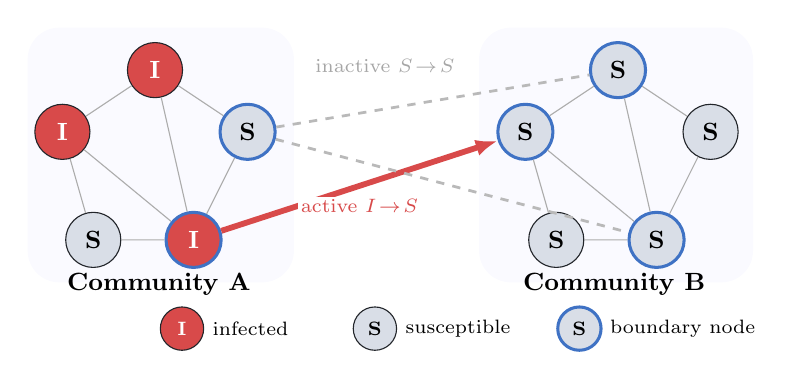
\begin{tikzpicture}[scale=0.98, every node/.style={font=\small}]
% Community backgrounds
\fill[blue!2,rounded corners=4mm] (-0.45,-0.55) rectangle (3.0,2.75);
\fill[blue!2,rounded corners=4mm] (5.4,-0.55) rectangle (8.95,2.75);
% A
\node[inode,text=white,font=\bfseries\small] (a1) at (0,1.4) {I};
\node[inode,text=white,font=\bfseries\small] (a2) at (1.2,2.2) {I};
\node[sbnode,font=\bfseries\small] (a3) at (2.4,1.4) {S};
\node[snode,font=\bfseries\small] (a4) at (0.4,0.0) {S};
\node[ibnode,text=white,font=\bfseries\small] (a5) at (1.7,0.0) {I};
\draw[gray!65] (a1)--(a2)--(a3)--(a5)--(a4)--(a1);
\draw[gray!65] (a1)--(a5); \draw[gray!65] (a2)--(a5);
\node[font=\bfseries\small] at (1.25,-0.58) {Community A};
% B
\node[sbnode,font=\bfseries\small] (b1) at (6.0,1.4) {S};
\node[sbnode,font=\bfseries\small] (b2) at (7.2,2.2) {S};
\node[snode,font=\bfseries\small] (b3) at (8.4,1.4) {S};
\node[snode,font=\bfseries\small] (b4) at (6.4,0.0) {S};
\node[sbnode,font=\bfseries\small] (b5) at (7.7,0.0) {S};
\draw[gray!65] (b1)--(b2)--(b3)--(b5)--(b4)--(b1);
\draw[gray!65] (b1)--(b5); \draw[gray!65] (b2)--(b5);
\node[font=\bfseries\small] at (7.15,-0.58) {Community B};
% cross edges: one currently active, two inactive
\draw[line width=2.1pt,infected,-{Latex[length=2.8mm]}] (a5)--node[below=1mm,fill=white,inner sep=1pt,font=\scriptsize,text=infected] {active $I\!\to\!S$} (b1);
\draw[line width=1.0pt,gray!55,dashed] (a3)--(b2);
\draw[line width=1.0pt,gray!55,dashed] (a3)--(b5);
\node[font=\scriptsize,text=gray!70] at (4.18,2.25) {inactive $S\!\to\!S$};
% legend
\node[inode,text=white,font=\bfseries\scriptsize,minimum size=5.5mm] at (1.55,-1.15) {I};
\node[anchor=west,font=\scriptsize] at (1.82,-1.15) {infected};
\node[snode,font=\bfseries\scriptsize,minimum size=5.5mm] at (4.05,-1.15) {S};
\node[anchor=west,font=\scriptsize] at (4.32,-1.15) {susceptible};
\node[sbnode,font=\bfseries\scriptsize,minimum size=5.5mm] at (6.70,-1.15) {S};
\node[anchor=west,font=\scriptsize] at (6.97,-1.15) {boundary node};
\end{tikzpicture}
\caption{Одна фізична мережа. Між communities є три реальні cross-edges, але зараз активне лише одне $I\to S$ ребро. Саме цю різницю між ``усіма ребрами'' та ``активними ребрами'' далі бачать або втрачають різні моделі.}
\end{figure}

Ця сама мережа буде подана всім симуляторам. Відмінність не в самій картинці, а в тому, \textbf{яку частину цієї картинки алгоритм використовує для міжcommunity передачі}.

\section*{2. Full Micro: алгоритм бачить усе}

Full Micro --- це повний Gillespie на всій мережі. Для нього немає принципової різниці між ``внутрішнім'' і ``міжcommunity'' ребром. Усі контакти --- це звичайні ребра одного графа.

Для кожного ребра $(u,v)$, де $u$ infected, а $v$ susceptible, існує канал зараження з rate
\[
 a_{uv}=\beta w_{uv}\,\I[X_u=I,\,X_v=S].
\]
Якщо ребра невагові, $w_{uv}=1$. Загальний infection hazard --- це сума rates усіх активних $I\to S$ ребер:
\[
 \Theta_{\text{micro}}=\sum_{(u,v)\in E} a_{uv}.
\]

Тобто Full Micro буквально запитує: ``\textit{Які конкретно заражені люди зараз мають контакт із конкретними susceptible людьми?}''

У мережі на рис. 1 між $A$ і $B$ є три фізичні ребра, але активне зараз тільки одне. Якщо всі мають rate $\beta$, точний міжcommunity hazard дорівнює
\[
 \lambda^{\text{exact}}_{AB}=\beta.
\]
Коли це ребро спрацьовує, заражається \textbf{саме той susceptible-вузол, який стоїть на його кінці}. Full Micro не вигадує target: його визначає реальне ребро.

\begin{tcolorbox}[colback=white,colframe=exact,title=Інтуїція]
Full Micro = ``я знаю стан кожної людини, кожне ребро і тому точно знаю, які переходи зараз можливі''.
\end{tcolorbox}

Це відповідає твоєму попередньому exact Gillespie-підходу на contact network: інтенсивність susceptible-вузла визначається його зараженими сусідами, а наступний event вибирається серед реально доступних transitions.

\section*{3. Original MicroMacro: детально всередині, грубо між communities}

MicroMacro робить головне спрощення: \textbf{усередині community він усе ще запускає локальний Gillespie на конкретних вузлах}, але між communities стискає інформацію.

Для macro-рівня community $A$ перетворюється приблизно на такий запис:
\[
 A:\quad I_A,\;S_A,\;N_A,
\]
а пара communities $A,B$ має агреговану вагу $W_{AB}$, яка описує силу їхнього зв'язку.

У твоїй MoMLeT-моделі міжcommunity rate записується як
\[
 \lambda_{AB}(t)=\beta\,W_{AB}\,C_A(t)\,S_B(t)\,T,
\]
де $C_A$ --- агрегована contagiousness source-community, а $S_B$ --- агрегована susceptibility destination-community. Для інтуїції це можна читати як схему
\[
 \lambda^{A/U}_{AB}\propto \beta W_{AB}\frac{I_A}{N_A}\frac{S_B}{N_B}.
\]

\begin{figure}[h!]
\centering
\begin{tikzpicture}[node distance=12mm,every node/.style={font=\small}]
\node[rounded corners=3mm,draw=boundary,line width=1.1pt,fill=blue!4,minimum width=43mm,minimum height=24mm,align=center] (A) {\textbf{Community A}\\$I_A=2,\;S_A=3$};
\node[rounded corners=3mm,draw=boundary,line width=1.1pt,fill=blue!4,minimum width=43mm,minimum height=24mm,align=center,right=48mm of A] (B) {\textbf{Community B}\\$I_B=0,\;S_B=5$};
\draw[-{Latex[length=3mm]},line width=2.2pt,macro] (A)--node[above=1mm,font=\bfseries] {$W_{AB}=3$} (B);
\node[draw=gray!55,dashed,rounded corners=2mm,fill=white,align=center,text width=43mm,below=8mm of A] (ha) {\textcolor{gray!70}{приховано:}\\які саме infected стоять на boundary};
\node[draw=gray!55,dashed,rounded corners=2mm,fill=white,align=center,text width=43mm,below=8mm of B] (hb) {\textcolor{gray!70}{приховано:}\\який susceptible є endpoint active edge};
\node[rounded corners=2mm,fill=macro!10,draw=macro,align=center,text width=48mm,below=6mm of $(ha)!0.5!(hb)$] {Macro бачить лише counts + $W_{AB}$, тому не відрізняє ``1 active edge'' від іншої конфігурації з тими самими агрегатами.};
\end{tikzpicture}
\caption{Macro-представлення тієї самої мережі. Локальні вузли не зникають із micro-models, але для міжcommunity hazard production MicroMacro використовує агреговані counts і $W_{AB}$, а не поточні стани конкретних cross-edges.}
\end{figure}

У нашому toy example $W_{AB}=3$ (три міжcommunity ребра), $I_A/N_A=2/5$, а $S_B/N_B=1$. Тоді агрегована формула може дати hazard близько
\[
 \lambda^{A/U}_{AB}=3\beta\cdot\frac{2}{5}=1.2\beta,
\]
хоча Full Micro бачить лише одне реально активне ребро і дає $\beta$.

Це і є \textbf{структурна апроксимація}: macro-рівень припускає, що infected і susceptible ``розмішані'' відносно boundary приблизно так само, як у всій community.

Коли macro-event відбувся, original MicroMacro не знає точний endpoint cross-edge. Тому він додає infection у \textbf{випадковий susceptible-вузол} destination-community.

\subsection*{3.1. Ще одна різниця: як MicroMacro рухає час}

Original MicroMacro не просто має aggregate hazard. Він має власний production scheduler. Micro communities просуваються блоками довжини $\tau_{\text{micro}}$, а macro-рівень накопичує hazard
\[
 H(t)=\int_{t_0}^{t}\Theta(s)\,ds
\]
до випадкового порогу $E=-\ln U$. У статті цей інтеграл апроксимується на micro-grid, зокрема через midpoint rate в кожному інтервалі.

\begin{figure}[h!]
\centering
\begin{tikzpicture}[every node/.style={font=\small}]
% Left: production scheduler
\node[font=\bfseries,text=macro] at (2.6,3.0) {Original MicroMacro};
\draw[->] (0,0.8)--(5.2,0.8) node[right] {$t$};
\foreach \x in {0,1.2,2.4,3.6,4.8} {\draw (\x,0.9)--(\x,0.7);}
\node[below,font=\scriptsize] at (1.2,0.72) {$\tau$};
\node[below,font=\scriptsize] at (2.4,0.72) {$2\tau$};
\node[below,font=\scriptsize] at (3.6,0.72) {$3\tau$};
\draw[macro,line width=1.8pt] (0,1.65)--(1.2,1.65)--(1.2,2.15)--(2.4,2.15)--(2.4,1.35)--(3.6,1.35)--(3.6,2.45)--(4.8,2.45);
\foreach \x/\y in {0.6/1.65,1.8/2.15,3.0/1.35,4.2/2.45} {\fill[macro] (\x,\y) circle (2pt);}
\node[align=center,text width=48mm,font=\scriptsize] at (2.5,-0.15) {Micro йде блоками $\tau$; macro hazard оцінюється на інтервалах і накопичується до випадкового threshold.};
% divider
\draw[gray!35,line width=0.8pt] (5.75,-0.45)--(5.75,3.2);
% Right: diagnostic direct competition
\node[font=\bfseries,text=purple] at (8.85,3.18) {Structural A/U diagnostic};
\draw[->] (6.35,0.8)--(11.2,0.8) node[right] {$t$};
\draw[line width=2pt,exact] (6.55,2.15)--(7.65,2.15);
\fill[exact] (7.65,2.15) circle (2.5pt);
\node[left,font=\scriptsize] at (6.55,2.15) {micro clock};
\node[above,font=\scriptsize] at (7.65,2.15) {$T_\mu=0.12$};
\draw[line width=2pt,macro] (6.55,1.45)--(9.95,1.45);
\fill[macro] (9.95,1.45) circle (2.5pt);
\node[left,font=\scriptsize] at (6.55,1.45) {macro clock};
\node[below,font=\scriptsize] at (9.95,1.45) {$T_M=0.37$};
\draw[-{Latex[length=2.4mm]},line width=1.2pt,purple] (7.65,2.35)--(7.65,2.62);
\node[above,font=\tiny,text=purple] at (7.65,2.62) {winner};
\node[align=center,text width=49mm,font=\scriptsize] at (8.75,-0.15) {На кожному state два exponential clocks конкурують напряму; після winner state оновлюється і rates рахуються знову.};
\end{tikzpicture}
\caption{Різниця scheduling. Production MicroMacro використовує $\tau$-синхронізацію та cumulative-hazard integration; A/U diagnostic залишає ту саму aggregate A/U ідею, але використовує direct event competition.}
\end{figure}

\section*{4. Structural A/U: ті самі грубі припущення, але інший simulator}

Оце найважливіший момент.

Structural A/U означає:
\[
 \boxed{A=\text{Aggregate hazard}},\qquad
 \boxed{U=\text{Uniform placement}}.
\]

Тобто за \textbf{структурним змістом} A/U робить те саме грубе припущення, що й original MicroMacro:
\begin{itemize}[nosep]
\item міжcommunity hazard рахується з агрегованої інформації, а не зі стану конкретних cross-edges;
\item після import заражається випадковий susceptible у destination-community.
\end{itemize}

Але A/U --- \textbf{не той самий executable code}. У diagnostic implementation немає production $\tau$-scheduler у тому самому вигляді. Там micro і macro події конкурують як event-driven stochastic clocks.

\begin{tcolorbox}[colback=soft,colframe=boundary,title=Навіщо взагалі потрібен A/U diagnostic?]
Від Full Micro original MicroMacro відрізняється одразу у двох місцях. По-перше, він замінює точні міжcommunity active edges на \textbf{aggregate hazard} і після import використовує \textbf{uniform placement}. По-друге, він використовує власний production $\tau$-scheduler замість прямої глобальної конкуренції подій.

A/U diagnostic залишає першу відмінність, але прибирає другу: \textbf{aggregate hazard + uniform placement залишаються, а production $\tau$-scheduler замінено на direct event competition}. Тому порівняння Full Micro з A/U показує переважно структурну похибку самої A/U-апроксимації, без домішки production synchronization mechanics.
\end{tcolorbox}

Тому різниця така:

\begin{center}
\begin{tabular}{>{\raggedright\arraybackslash}p{42mm} >{\raggedright\arraybackslash}p{52mm} >{\raggedright\arraybackslash}p{52mm}}
\toprule
 & \textbf{Original MicroMacro} & \textbf{Structural A/U}\\
\midrule
Macro information & aggregate & aggregate\\
Placement & uniform susceptible & uniform susceptible\\
Hazard idea & та сама A/U approximation & та сама A/U approximation\\
Time scheduler & production $\tau$ + hazard integral & окремий event-driven scheduler\\
Executable & original user-facing simulator & окремий diagnostic simulator\\
\bottomrule
\end{tabular}
\end{center}

Отже відповідь на питання ``\textit{чи hazard рахується інакше?}'' така:

\begin{tcolorbox}[colback=soft,colframe=macro,title=Коротка відповідь]
У A/U \textbf{не обов'язково інша structural formula hazard}; за змістом вона така сама aggregate approximation, як у MicroMacro. Головна відмінність A/U від original MicroMacro --- \textbf{не formula, а simulation scheduler та implementation mechanics}. Саме тому A/U потрібен, щоб подивитися на ``чисту'' structural approximation без частини production implementation artifacts.
\end{tcolorbox}

\subsection*{4.1. Що показало порівняння A/U з Full Micro і MicroMacro}

Числа нижче --- для одного й того самого baseline: 100 paired мереж, $L=10$, $n=100$, $d\approx6$, $k=5$, $\beta_{\mathrm{in}}=\beta_{\mathrm{out}}=0.003$, SI, $T_{\mathrm{end}}=4000$. Основна метрика --- RMST до досягнення останньої community: більший RMST означає \textbf{повільніше} проходження інфекції вздовж ланцюга.

\subsubsection*{Що таке RMST і як він тут рахується}

RMST --- це \textit{Restricted Mean Survival Time}, тобто середній час до події, але з фіксованим максимальним горизонтом спостереження. У цьому експерименті ``подія'' --- \textbf{перше досягнення інфекцією останньої community} в ланцюгу. Для replication $r$ позначимо цей час як $T_{\mathrm{last}}^{(r)}$. Якщо остання community досягнута до кінця симуляції, беремо фактичний час. Якщо ні, replication не викидається: її внесок обмежується горизонтом $T_{\mathrm{end}}=4000$.

Для $R$ replications:
\[
\mathrm{RMST}
=\frac{1}{R}\sum_{r=1}^{R}
\min\!\left(T_{\mathrm{last}}^{(r)},T_{\mathrm{end}}\right).
\]

Наприклад, якщо три runs дали terminal arrival $2800$, $3200$ і ``не досягнуто до 4000'', то в середнє входять $2800$, $3200$ і $4000$:
\[
\mathrm{RMST}=\frac{2800+3200+4000}{3}=3333.3.
\]
Якщо всі runs завершилися до горизонту, RMST тут просто збігається зі звичайним середнім $T_{\mathrm{last}}$. \textbf{Більший RMST} означає пізніше проходження інфекції до кінця chain, тобто повільнішу propagation. У таблицях
\[
\Delta\mathrm{RMST}=\mathrm{RMST}_{\mathrm{variant}}-\mathrm{RMST}_{\mathrm{Full\ Micro}}.
\]
Тому від'ємне $\Delta$ означає, що variant доходить до останньої community раніше за Full Micro, а додатне --- пізніше.

\begin{center}
\begin{tabular}{l r r}
\toprule
\textbf{Simulator} & \textbf{RMST} & \textbf{$\Delta$ vs Full Micro}\\
\midrule
Full Micro & 2936.73 & 0\\
Structural A/U & 2715.94 & $-220.79$\\
Original MicroMacro, current Production ($\tau=1$) & 1677.55 & $-1259.18$\\
Production + independent RNG streams & 2729.43 & $-207.30$\\
\bottomrule
\end{tabular}
\end{center}

A/U приходить до кінця в середньому приблизно на \textbf{221 одиницю часу раніше}, ніж Full Micro ($\Delta\mathrm{RMST}=-220.8$; 95\% CI приблизно $[-315.5,-126.8]$). Це і є чистий сигнал, що навіть без production scheduler aggregate hazard + uniform placement уже дають систематичне прискорення.

Водночас current Production MicroMacro був ще набагато швидшим: RMST $1677.55$. Різниця між ним і event-driven A/U становила близько \textbf{1038 RMST}. Але цей великий gap \textbf{не можна приписувати самому $\tau$-scheduler}. Після виправлення shared-RNG architecture Production дав RMST $2729.43$ і відрізнявся від A/U лише на $+13.49$ RMST; 95\% CI цього contrast включає нуль. Окремо зменшення $\tau$ від $1$ до $0.25$ змінювало RMST лише приблизно на $31.15$.


\subsubsection*{Що означають ``current Production'' і ``Production + independent RNG streams''}

Це \textbf{не дві різні наукові моделі}. Обидва варіанти використовують той самий production MicroMacro: ті самі community MicroModels, aggregate macro hazard, uniform import placement, $\tau=1$, midpoint/cumulative-hazard scheduler і normal repeated imports. У variant ``Production + independent RNG streams'' змінено лише те, \textbf{звідки кожна micro-community бере випадкові числа}.

У current Production кожен \texttt{MicroModel} створюється без власного RNG. Тоді всі communities використовують один і той самий module-level Python \texttt{random}, тобто \textbf{один спільний RNG state}. Сам по собі один спільний pseudorandom generator ще не був би помилкою. Проблема виникає через комбінацію \textbf{shared RNG + horizon-safe rollback}.

Коли \texttt{simulate\_until(t\_end)} пробує наступну Gillespie event і бачить, що її час лежить за поточним horizon, він повертає RNG у стан \texttt{rng\_before}. Для окремого RNG це локальна операція. Але в current Production цей state є глобальним для всіх communities. Тому rollback однієї community повертає назад random stream також для наступної community, яка симулюється після неї.

\begin{tcolorbox}[colback=soft,colframe=macro,title=Чому з'являється штучна залежність]
Уявімо, що перед симуляцією community A глобальний RNG має стан $R$. A генерує random draw, але event лежить за horizon, тому код відновлює state назад до $R$. Потім симулюється community B. Вона стартує з того самого $R$ і може повторно використати ту саму послідовність random draws. Отже stochastic evolution B починає залежати від того, як A просувалася до horizon і чи зробила rollback. Це \textbf{cross-community RNG coupling та order dependence}, а не фізичний зв'язок між communities.
\end{tcolorbox}

У correction variant кожній micro-community явно призначається власний generator,
\[
\mathrm{RNG}_1,\mathrm{RNG}_2,\ldots,\mathrm{RNG}_L,
\]
з окремим deterministic seed. Тоді rollback community $i$ змінює тільки state $\mathrm{RNG}_i$ і не може повернути random stream іншої community. Midpoint clones також копіюють/відновлюють саме per-community RNG state. Macro budget і pair selection при цьому залишаються частиною original production machinery; scientific aggregate A/U semantics та $\tau$-scheduler не змінюються.

Окремий unit diagnostic підтвердив, що це не лише теоретична можливість. Для двох однакових ізольованих micro-processes shared-global mode дав correlation фінальних infected counts приблизно $0.531$; для independent streams --- $-0.002$. Ще сильніший сигнал: імовірність заразити target у першої community була $0.394$, а у другої лише $0.155$ при shared RNG. Після розділення streams значення стали приблизно $0.394$ і $0.390$. Тобто shared RNG + rollback змінював навіть marginal distribution другої community.

\begin{center}
\small
\begin{tabular}{p{31mm} p{42mm} p{42mm} p{42mm}}
\toprule
\textbf{Implementation} & \textbf{Micro scheduling / state} & \textbf{Cross-community model} & \textbf{RNG architecture}\\
\midrule
Full Micro & один global Gillespie process на full graph & exact active edges, exact endpoint & один RNG для одного global process\\
Current Production MM & окремі MicroModels + $\tau$-synchronization & aggregate hazard + uniform import & один shared global RNG між micro communities\\
Production + independent RNG & \textbf{той самий production scheduler} & \textbf{та сама aggregate/uniform model} & окремий RNG для кожної micro-community\\
Structural A/U & один diagnostic global node state, event-driven race & aggregate hazard + uniform placement & окремі streams за stochastic roles; не production scheduler\\
E/U, E/E & той самий diagnostic event-driven framework & exact hazard; E/U uniform, E/E exact placement & diagnostic streams, не production per-community architecture\\
\bottomrule
\end{tabular}
\end{center}

Тому назва ``Production + independent RNG streams'' означає саме \textbf{мінімальну implementation correction original MicroMacro}, а не новий E/U/E/E simulator. Її призначення --- перевірити, що станеться, якщо зберегти production algorithm, але прибрати штучне stochastic coupling між локальними micro-simulators.

\begin{tcolorbox}[colback=soft,colframe=macro,title=Як це читати]
\textbf{Full Micro $\to$ A/U} показує головним чином structural A/U error.\newline
\textbf{A/U $\to$ current Production MicroMacro} у цій версії показував переважно implementation/RNG problem, а не ``похибку від $\tau$'' як таку. Після RNG correction production і A/U практично збіглися.
\end{tcolorbox}

\section*{5. E/U: виправляємо тільки hazard}

Тепер ми залишаємо uniform placement, але повертаємо точну інформацію про реальні міжcommunity ребра.

Для pair $A\to B$ exact hazard:
\[
 \lambda^{E/U}_{AB}
 =\beta\sum_{(u,v)\in E_{AB}} w_{uv}\,\I[X_u=I,\,X_v=S].
\]

У toy network з рис. 1 активне тільки одне cross-edge, тому
\[
 \lambda^{E/U}_{AB}=\beta,
\]
а не $1.2\beta$, як у нашому простому aggregate прикладі.

Але після того, як macro-event відбувся, E/U все ще робить ``U'': вибирає \textbf{будь-який susceptible} у $B$, а не обов'язково endpoint активного ребра.

\begin{figure}[h!]
\centering
\begin{tikzpicture}[every node/.style={font=\small}]
% Stage 1 exact hazard
\node[font=\bfseries\small,text=exact,align=center] at (1.75,2.15) {1. Exact hazard\\``коли?''};
\node[ibnode,text=white,font=\bfseries\small] (a) at (0.25,0.9) {I};
\node[sbnode,font=\bfseries\small] (b1) at (3.8,0.9) {S};
\node[sbnode,font=\bfseries\small] (b2) at (3.8,1.7) {S};
\node[sbnode,font=\bfseries\small] (b3) at (3.8,0.1) {S};
\draw[exact,line width=2.3pt,-{Latex[length=2.8mm]}] (a)--node[above,font=\scriptsize] {active $I\to S$} (b1);
\draw[gray!50,dashed] (0.25,0.9)--(b2);
\draw[gray!50,dashed] (0.25,0.9)--(b3);
\node[align=center,text width=43mm,font=\scriptsize] at (2.05,-0.55) {У hazard входить лише реально активне cross-edge. Неактивні контакти не додають rate.};
% Transition
\draw[-{Latex[length=3mm]},line width=1.4pt,purple] (4.45,0.9)--(5.3,0.9);
\node[above,font=\scriptsize,text=purple] at (4.88,0.9) {event};
% Stage 2 uniform placement
\node[font=\bfseries\small,text=purple,align=center] at (8.05,2.15) {2. Uniform placement\\``куди?''};
\node[snode,font=\bfseries\small] (u1) at (6.1,1.20) {S};
\node[snode,font=\bfseries\small] (u2) at (7.35,1.40) {S};
\node[snode,font=\bfseries\small] (u3) at (8.6,1.20) {S};
\node[snode,font=\bfseries\small] (u4) at (6.65,0.15) {S};
\node[snode,font=\bfseries\small] (u5) at (8.05,0.15) {S};
\foreach \n in {u1,u2,u3,u4,u5} {\draw[purple,line width=1pt] (\n) circle (5.3mm);}
\node[align=center,text width=45mm,font=\scriptsize] at (7.35,-0.72) {Після macro-event E/U усе ще вибирає target uniformly серед усіх susceptible destination-community.};
\end{tikzpicture}
\caption{E/U виправляє тільки hazard. Він точно визначає інтенсивність міжcommunity передачі з active edges, але placement після event залишається uniform.}
\end{figure}

Тому перехід A/U $\to$ E/U вимірює насамперед помилку від \textbf{aggregate hazard}. Обидва варіанти запускаються тим самим diagnostic event-driven scheduler і в обох placement залишається uniform. Змінюється лише джерело macro hazard: у A/U він агрегований, а в E/U рахується з реальних active $I\to S$ cross-edges.

\begin{tcolorbox}[colback=white,colframe=purple,title=Що саме перевіряє E/U?]
Якщо E/U стає помітно ближчим до Full Micro, ніж A/U, це означає, що значна частина structural error виникала через \textbf{втрату інформації про те, які міжcommunity ребра реально активні}. Scheduler тут не міняється, тому його вплив не плутається з ефектом exact hazard.
\end{tcolorbox}

\subsection*{5.1. Що показало порівняння E/U з Full Micro і MicroMacro}

На тому самому baseline E/U дав:

\begin{center}
\begin{tabular}{l r r}
\toprule
\textbf{Simulator} & \textbf{RMST} & \textbf{$\Delta$ vs Full Micro}\\
\midrule
Full Micro & 2936.73 & 0\\
Structural E/U & 2775.5 & $-161.2$\\
Structural A/U & 2715.94 & $-220.79$\\
Original MicroMacro, current Production & 1677.55 & $-1259.18$\\
\bottomrule
\end{tabular}
\end{center}

Після заміни aggregate hazard на exact active-edge hazard RMST зріс приблизно на \textbf{59.6} відносно A/U. Тобто E/U рухається в правильний бік --- ближче до Full Micro. Але від Full Micro все ще залишається значущий gap: приблизно $-161.2$ RMST, 95\% CI $[-266.8,-48.8]$.

Причина проста: E/U уже правильно знає \textit{коли} міжcommunity infection може відбутися, але після event усе ще може покласти infection у неправильне місце, бо target залишається uniform.

Порівняно з current Production MicroMacro E/U має RMST приблизно на \textbf{1098} більший. Цей raw gap не слід трактувати як ``ефект exact hazard'': current Production baseline містив великий shared-RNG implementation defect. Інформативніше дивитися на послідовність A/U $\to$ E/U, де scheduler однаковий і змінюється тільки hazard.

\begin{tcolorbox}[colback=soft,colframe=purple,title=Головний результат E/U]
Exact hazard \textbf{частково} повертає поведінку до Full Micro, але не закриває весь structural gap. Отже знати лише правильну сумарну інтенсивність недостатньо: важливо ще й правильно визначити, \textit{який} вузол у destination-community отримує import.
\end{tcolorbox}

\section*{6. E/E: виправляємо і hazard, і placement}

E/E означає:
\[
 \boxed{E=\text{Exact hazard}},\qquad
 \boxed{E=\text{Exact placement}}.
\]

Hazard такий самий exact active-edge sum, як в E/U. Але тепер, якщо event вибрано через конкретне ребро $(u,v)$, заражається саме його endpoint $v$.

Тобто E/E знає обидві речі:
\begin{enumerate}[nosep]
\item \textbf{як часто} має відбуватися inter-community transmission;
\item \textbf{куди саме} він може потрапити.
\end{enumerate}

Перехід E/U $\to$ E/E ізолює помилку від \textbf{uniform placement}. Scheduler і exact hazard залишаються такими самими, як в E/U; змінюється лише правило вибору target-вузла після міжcommunity event.

\begin{tcolorbox}[colback=white,colframe=exact,title=Що саме перевіряє E/E?]
E/E відповідає на питання: ``якщо ми вже правильно знаємо \textit{коли} має відбутися міжcommunity зараження, скільки ще похибки дає те, що MicroMacro не знає \textit{який саме} вузол має заразитися?'' Якщо E/E майже збігається з Full Micro, це також є sanity check, що diagnostic event-driven implementation правильно відтворює exact process, коли йому повернули всю потрібну edge-level інформацію.
\end{tcolorbox}

\subsection*{6.1. Що показало порівняння E/E з Full Micro і MicroMacro}

Результат E/E був майже таким самим, як Full Micro:

\begin{center}
\begin{tabular}{l r r}
\toprule
\textbf{Simulator} & \textbf{RMST} & \textbf{$\Delta$ vs Full Micro}\\
\midrule
Full Micro & 2936.73 & 0\\
Structural E/E & 2944.3 & $+7.5$\\
Structural E/U & 2775.5 & $-161.2$\\
Original MicroMacro, current Production & 1677.55 & $-1259.18$\\
\bottomrule
\end{tabular}
\end{center}

Різниця E/E vs Full Micro становила лише $+7.5$ RMST, а 95\% CI $[-93.6,+120.3]$ включав нуль. Тобто в цьому baseline немає статистичних підстав вважати, що E/E систематично відрізняється від Full Micro.

Перехід E/U $\to$ E/E дав приблизно \textbf{+168.8 RMST} (тобто propagation стала пізнішою і ближчою до Full Micro); відповідний 95\% CI для improvement приблизно $[56.1,274.5]$. Це показує, що при вже правильному hazard саме placement був великим залишковим джерелом structural error.

Порівняно з current Production MicroMacro E/E має RMST приблизно на \textbf{1267} більший. Тут це очікувано: E/E уже повертає exact edge-level information і тому поводиться як Full Micro, тоді як current Production мав одночасно structural approximation та implementation defect.

\begin{tcolorbox}[colback=soft,colframe=exact,title=Головний результат E/E]
У цьому baseline E/E практично відтворює Full Micro. Це сильний sanity check: коли diagnostic simulator отримує exact hazard і exact target, різниця з глобальним Full Micro зникає в межах Monte-Carlo uncertainty.
\end{tcolorbox}

\section*{7. То яка різниця між E/E і Full Micro?}

Після перевірки реалізацій тут можна сказати точніше: \textbf{у Experiment 01 E/E і Full Micro налаштовані так, щоб задавати той самий CTMC generator}. Вони відрізняються не правилами зараження, а способом, яким одна й та сама множина подій організована та вибирається в коді.

\textbf{Full Micro} отримує весь \texttt{full\_graph} і передає його одному \texttt{MicroEngine}. Для нього внутрішнє ребро і cross-community edge --- просто два ребра одного графа. Кожне активне ребро $u(I)-v(S)$ дає infection channel
\[
 a_{uv}=\beta w_{uv},
\]
а recovery кожного infected-вузла має rate $\gamma$. Усі infection та recovery channels входять в одну Gillespie competition.

\textbf{E/E} також працює з одним глобальним станом усіх вузлів. Важливо: у ньому немає окремого ``micro A simulator'' і ``micro B simulator''. Код лише \textbf{індексує ребра двома групами}: internal edges та cross-community edges. Для internal активного $I-S$ ребра використовується $\beta_{\mathrm{in}}w$; для cross-community активного $I-S$ ребра --- $\beta_{\mathrm{out}}w$.

У runner цього експерименту є явна перевірка
\[
\beta_{\mathrm{in}}=\beta_{\mathrm{out}},
\]
оскільки Full Micro має один infection rate для всіх ребер. Тому в Experiment 01 відповідне активне ребро має \textbf{той самий rate} у Full Micro та E/E. Recovery rule також однаковий: кожний infected-вузол має rate $\gamma$.

\begin{figure}[h!]
\centering
\begin{tikzpicture}[every node/.style={font=\small},scale=0.91]
% Full Micro
\node[font=\bfseries,text=exact] at (2.25,2.7) {Full Micro};
\fill[green!3,rounded corners=3mm] (-0.35,-0.75) rectangle (4.85,2.35);
\node[inode,text=white,font=\bfseries\scriptsize,minimum size=6mm] (f1) at (0.25,1.55) {I};
\node[snode,font=\bfseries\scriptsize,minimum size=6mm] (f2) at (1.45,1.95) {S};
\node[inode,text=white,font=\bfseries\scriptsize,minimum size=6mm] (f3) at (1.3,0.55) {I};
\node[sbnode,font=\bfseries\scriptsize,minimum size=6mm] (f4) at (3.55,1.45) {S};
\node[snode,font=\bfseries\scriptsize,minimum size=6mm] (f5) at (4.3,0.55) {S};
\draw[gray!60] (f1)--(f2)--(f3)--(f1);
\draw[gray!60] (f4)--(f5);
\draw[exact,line width=2.1pt,-{Latex[length=2.5mm]}] (f3)--(f4);
\node[font=\tiny,align=center,text width=49mm] at (2.25,-0.26) {усі active channels $\Downarrow$ одна global Gillespie race};

% E/E
\node[font=\bfseries,text=purple] at (8.05,2.7) {E/E diagnostic};
\fill[purple!3,rounded corners=3mm] (5.45,-0.75) rectangle (10.7,2.35);
\node[inode,text=white,font=\bfseries\scriptsize,minimum size=6mm] (e1) at (5.95,1.55) {I};
\node[snode,font=\bfseries\scriptsize,minimum size=6mm] (e2) at (7.0,1.95) {S};
\node[ibnode,text=white,font=\bfseries\scriptsize,minimum size=6mm] (e3) at (6.95,0.55) {I};
\node[sbnode,font=\bfseries\scriptsize,minimum size=6mm] (e4) at (8.85,1.45) {S};
\node[snode,font=\bfseries\scriptsize,minimum size=6mm] (e5) at (9.8,0.55) {S};
\draw[gray!60] (e1)--(e2)--(e3)--(e1);
\draw[gray!60] (e4)--(e5);
\draw[exact,line width=2.1pt,-{Latex[length=2.5mm]}] (e3)--(e4);
\node[font=\tiny,align=center,text width=50mm] at (8.05,-0.28) {ті самі channels, але згруповані: internal+recovery vs cross-edge clock};

\draw[<->,line width=1.2pt,dark] (4.9,1.05)--(5.4,1.05);
\node[font=\tiny,fill=white,inner sep=1pt,align=center] at (5.15,0.7) {same CTMC\\generator};
\end{tikzpicture}
\caption{У Experiment 01 E/E не має окремих micro-simulators для communities. Він має один глобальний node state, але програмно групує event channels на internal/recovery та cross-community. Full Micro тримає всі ці channels в одній Gillespie race.}
\end{figure}

\textbf{Чому дві групи clocks не змінюють процес?} Нехай
\[
\Lambda_{\mu}=\Lambda_{\mathrm{internal}}+\Lambda_{\mathrm{recovery}},
\qquad
\Lambda_{M}=\Lambda_{\mathrm{cross}}.
\]
Full Micro генерує один час
\[
\Delta t\sim \mathrm{Exp}(\Lambda_{\mu}+\Lambda_M).
\]
E/E генерує два незалежні часи
\[
T_{\mu}\sim\mathrm{Exp}(\Lambda_{\mu}),\qquad
T_M\sim\mathrm{Exp}(\Lambda_M)
\]
і бере найменший. Для exponential clocks
\[
\min(T_{\mu},T_M)\sim\mathrm{Exp}(\Lambda_{\mu}+\Lambda_M),
\]
а ймовірність перемоги кожної групи пропорційна її rate. Тому така дворівнева організація sampling математично еквівалентна одній глобальній Gillespie race.

Для cross-community event E/E також зберігає точні ймовірності конкретних активних ребер. Спочатку pair $i\to j$ вибирається пропорційно сумі rates його активних cross-edges. Потім target вибирається пропорційно сумі ваг активних ребер, що входять у нього, а source --- пропорційно вазі відповідного active edge. У результаті конкретне ребро $(u,v)$ вибирається з тією самою ймовірністю, що й у Full Micro.

\begin{tcolorbox}[colback=soft,colframe=exact,title={Отже, тут не треба писати ``if rules match''}]
Для конфігурації Experiment 01 умови еквівалентності \textbf{перевірені самою реалізацією}: той самий full graph та initial node, $\beta_{\mathrm{in}}=\beta_{\mathrm{out}}$, той самий $\gamma$, ті самі SIR event rules, exact active cross-edge hazard і exact edge-conditioned placement. Тому E/E та Full Micro повинні мати один статистичний розподіл, хоча конкретні trajectories різняться через іншу організацію RNG streams.
\end{tcolorbox}

Саме це перевіряє oracle gate. У 100 paired replications Full Micro мав RMST $2936.7$, E/E --- $2944.3$; різниця $+7.5$ з 95\% CI $[-93.6,+120.3]$. Інтервал містить нуль, тобто дані не показують систематичної різниці між двома реалізаціями. Це узгоджується з перевіркою коду: E/E є альтернативною реалізацією того самого CTMC, а не ще однією approximation.

\textit{Перевірено за реалізаціями:} \texttt{simulators/micro.py}, \texttt{engines/micro\_engine.py},\\
\texttt{hazard\_placement\_ablation/simulator.py} та \texttt{hazard\_placement\_ablation/runner.py}.

\section*{8. Уся логіка A/U $\to$ E/U $\to$ E/E одним ланцюжком}

Перед самим ablation ladder корисно тримати в голові дві різні причини, чому original MicroMacro може відрізнятися від Full Micro:
\begin{center}
\begin{tabular}{>{\raggedright\arraybackslash}p{29mm} >{\raggedright\arraybackslash}p{112mm}}
\textbf{Structural:} & exact boundary edges $\to$ aggregate community hazard.\\[2pt]
\textbf{Scheduler:} & global event competition $\to$ $\tau$-synchronized hazard integration.
\end{tabular}
\end{center}
A/U diagnostic спеціально прибирає другу різницю, але залишає першу. Далі A/U $\to$ E/U повертає exact hazard, а E/U $\to$ E/E повертає exact placement.


\begin{center}
\begin{tabular}{l r r r}
\toprule
\textbf{Variant} & \textbf{RMST} & \textbf{$\Delta$ vs Full Micro} & \textbf{$\Delta$ vs current MM}\\
\midrule
Current Production MicroMacro & 1677.55 & $-1259.18$ & 0\\
A/U & 2715.94 & $-220.79$ & $+1038.39$\\
E/U & 2775.5 & $-161.2$ & $+1098.0$\\
E/E & 2944.3 & $+7.5$ & $+1266.8$\\
Full Micro & 2936.73 & 0 & $+1259.18$\\
\bottomrule
\end{tabular}
\end{center}

Ця таблиця добре показує дві різні історії. Великий стрибок від current Production до A/U був переважно implementation/RNG correction, тоді як подальші кроки A/U $\to$ E/U $\to$ E/E уже послідовно повертають structural information і ведуть diagnostic model до Full Micro.

\begin{figure}[h!]
\centering
\begin{tikzpicture}[node distance=9mm and 7mm,every node/.style={font=\small}]
% production baseline on top
\node[rounded corners=2mm,draw=macro,line width=1.1pt,fill=macro!8,text width=49mm,minimum height=18mm,align=center] (prod) {\textbf{Original MicroMacro}\\aggregate hazard + uniform target\\$\tau$-synchronized scheduler};
\node[rounded corners=2mm,draw=macro,fill=macro!4,text width=35mm,minimum height=18mm,align=center,below=13mm of prod] (au) {\textbf{A/U}\\aggregate hazard\\uniform target};
\draw[-{Latex[length=3mm]},line width=1.4pt,purple] (prod)--node[right=3mm,yshift=2mm,font=\scriptsize,align=left,text width=43mm] {прибираємо тільки production $\tau$-scheduler; structural assumptions лишаються} (au);
% diagnostic ladder
\node[rounded corners=2mm,draw=purple,fill=purple!7,text width=35mm,minimum height=18mm,align=center,right=18mm of au] (eu) {\textbf{E/U}\\exact hazard\\uniform target};
\node[rounded corners=2mm,draw=exact,fill=green!7,text width=35mm,minimum height=18mm,align=center,right=18mm of eu] (ee) {\textbf{E/E}\\exact hazard\\exact target};
\draw[-{Latex[length=3mm]},line width=1.4pt] (au)--node[above,font=\scriptsize,align=center] {міняємо тільки\\hazard} (eu);
\draw[-{Latex[length=3mm]},line width=1.4pt] (eu)--node[above,font=\scriptsize,align=center] {міняємо тільки\\placement} (ee);
% Full Micro sanity target
\node[rounded corners=2mm,draw=exact,dashed,fill=green!3,text width=35mm,minimum height=16mm,align=center,below=12mm of ee] (full) {\textbf{Full Micro}\\exact global CTMC};
\draw[-{Latex[length=3mm]},dashed,line width=1.1pt,exact] (ee)--node[right=2mm,font=\scriptsize,align=left,text width=38mm] {sanity check: той самий distribution, якщо exact rules збігаються} (full);
% takeaways
\node[below=11mm of au,align=center,text width=38mm,font=\scriptsize] {Full Micro vs A/U:\\переважно \textbf{structural A/U error}.};
\node[below=11mm of eu,align=center,text width=39mm,font=\scriptsize] {A/U $\to$ E/U:\\\textbf{aggregate-hazard error}.};
\end{tikzpicture}
\caption{Що саме ізолює кожен крок. A/U відділяє structural assumptions від production scheduling; E/U змінює лише hazard; E/E змінює лише placement і служить sanity check проти Full Micro.}
\end{figure}

\section*{9. Що вважати основним результатом для статті}

Тут важливе методологічне правило.

Якщо ми хочемо сказати щось саме про \textbf{твій user-facing MicroMacro method}, primary experiments краще робити на original `MicroMacroSimulator` і змінювати мінімально необхідну деталь:

\begin{center}
\begin{tabular}{p{35mm} p{107mm}}
\toprule
\textbf{Experiment} & \textbf{Найчистіша реалізація}\\
\midrule
A/U baseline & original MicroMacro без змін\\
E/U & original MicroMacro + замінити лише macro hazard provider на exact active-edge hazard\\
E/E & те саме + замінити лише target selector на exact edge endpoint\\
Gateway near/random/far & simulator взагалі не змінювати; змінювати тільки topology\\
$d\times k$ grid & simulator не змінювати; змінювати лише параметри мережі\\
\bottomrule
\end{tabular}
\end{center}

Окремий `HazardPlacementSimulator` все одно корисний: він дуже добре підходить як \textbf{secondary mechanistic diagnostic}, бо прибирає production scheduler artifacts і дозволяє чисто розкласти structural error. Але його результати краще подавати як підтвердження механізму, а не як єдине свідчення того, що отримає користувач original MicroMacro.

\section*{10. Найкоротше резюме}

\begin{tcolorbox}[colback=soft,colframe=dark]
\textbf{Full Micro:} бачить кожен вузол і кожне active edge. Exact hazard, exact target.\\[3pt]
\textbf{Original MicroMacro:} усередині community бачить nodes, між communities бачить aggregate $I,S,W$. Aggregate hazard, uniform target, production $\tau$-scheduler.\\[3pt]
\textbf{Structural A/U:} ті самі aggregate/uniform structural assumptions, але окремий event-driven diagnostic simulator; тому він прибирає production $\tau$-scheduler і залишає structural A/U approximation.\\[3pt]
\textbf{E/U:} той самий diagnostic scheduler і той самий uniform placement, але aggregate hazard замінено на exact cross-edge hazard; різниця A/U $\to$ E/U ізолює hazard information loss.\\[3pt]
\textbf{E/E:} той самий diagnostic scheduler та exact hazard, але uniform placement замінено на exact endpoint; різниця E/U $\to$ E/E ізолює placement error. Якщо решта event rules збігаються з Full Micro, статистично має відтворювати той самий CTMC.
\end{tcolorbox}

\section*{Примітка про джерела}
Опис original MicroMacro, його двох рівнів, macro-rate та cumulative-hazard synchronization базується на наданій роботі \textit{Towards complexity reduction of large-scale epidemic simulation in two-scale networks} (MoMLeT-2025). Опис Full Micro спирається на надану роботу \textit{Simulating epidemic peak dynamics on complex networks using efficient Gillespie algorithms}. Розрізнення Structural A/U--E/U--E/E як окремої diagnostic implementation базується на перевіреному source code експериментів у Google Drive в межах поточного аудиту. Числові результати RMST взято з Experiment 01 (factorial hazard/placement ablation, 31.07.2026, 100 paired replications) та Experiment 07 (production implementation decomposition, аналіз 14.08.2026).

\end{document}
